\documentclass{beamer}

\mode<presentation> {
	\usetheme{Boadilla}
	%\usetheme{CambridgeUS}
}
\usefonttheme[onlymath]{serif}
\usepackage{graphicx}
\usepackage{booktabs} % Allows the use of \toprule, \midrule and \bottomrule in tables
\usepackage{amssymb,mathrsfs,amsmath}
\usepackage{bbding}
\usepackage{amsfonts}
\usepackage{enumerate}
\usepackage{color}
\usepackage{xcolor}
%-------------------------------------------------------------------------

\title[Firms in the open economy]{Firms in the open economy \\ {\small A review}}
\author{Qinzhu Sun} 
\institute[]{}

\date{April 15, 2022}
\logo{
\includegraphics[scale=0.2]{maingate2}}
\begin{document}

\begin{frame}
	\titlepage
\end{frame}

\begin{frame}{Overview}
	\tableofcontents
\end{frame}
%-------------------------------------------------------------------------
%-------------------------------------------------------------------------
\section{Introduction}
\begin{frame}[shrink]
	\transfade %fade in and fade out
	\tableofcontents[sectionstyle=show/shaded,subsectionstyle=show/shaded/hide]
	\addtocounter{framenumber}{-1}
\end{frame}
%------------------------------------------------
\begin{frame}{Trade theory and stylized facts}
	\textbf{Gains from inter-industry specialization}
	\begin{itemize}
		\item Focus: Inter-industry trade
		\item Theory: Comparative advantage (David Ricardo, \dots)
	\end{itemize}
	\textbf{Gains from intra-industry specialization}
	\begin{itemize}
		\item Focus: Intra-industry trade
		\item Theory: Scale economy, love-for-variety (Krugman 1980)
	\end{itemize}
	\textbf{Gains from inter-firm specialization}
	\begin{itemize}
		\item Focus: Firm heterogeneity
		\item Theory: Reallocation effect, procompetitive effect, etc. (Melitz 2003, Melitz \& Ottaviano 2008)
	\end{itemize}
	\textbf{Gains from within-firm specialization}
	\begin{itemize}
		\item Focus: Fragmentation, factor matching, MNE boundaries
		\item Theory: Transaction cost, span of control, contract theory (Coase 1937, Lucas 1978, Grossman \& Hart 1986, Antr\`as et al. 2006)
	\end{itemize}
\end{frame}
%------------------------------------------------
\begin{frame}{Firm heterogeneity}
	Traditional trade theories usually simply assumes \textcolor{red}{a representative firm} within each industry.
	\medskip

	\textbf{Phenomenon}
	\begin{itemize}
		\item Firm participation in international trade is exceedingly \textcolor{red}{rare}.
		\item Ex(Im)porters and non-ex(im)porters are \textcolor{red}{different}.
	\end{itemize}
	\medskip

	\textbf{Mechanism}
	\begin{itemize}
		\item Reallocation effect (Melitz 2003)
		\item Procompetitive effect (Bernard et al. 2003, Melitz \& Ottaviano 2008)
		\item Productivity effect (Pavcnik 2002, Trefler 2004)
		\item etc.
	\end{itemize}
\end{frame}
%-------------------------------------------------------------------------
%-------------------------------------------------------------------------
\section{Firm Organization Problem}
\begin{frame}[shrink]
	\transfade %fade in and fade out
	\tableofcontents[sectionstyle=show/shaded,subsectionstyle=show/shaded/hide]
	\addtocounter{framenumber}{-1}
\end{frame}
%------------------------------------------------
\subsection{Fragmentation in otherwise Neoclassical Models}
\begin{frame}[shrink]
	\transfade %fade in and fade out
	\tableofcontents[sectionstyle=show/shaded,subsectionstyle=show/shaded/hide]
	\addtocounter{framenumber}{-1}
\end{frame}
%------------------------------------------------
\begin{frame}{Unbundling the production process / Fragmentation}
	Suppose firm $n$ produces output $y_i(n)$ by completing a set of $M_i(n)$ tasks. Let $T_i$ be the scale of task $i$. Assume the firm's output to be
	\begin{equation}
		y_i(n)=f_{i,n}(T_1,T_2,...,T_{M_i}).
	\end{equation}
	\medskip
	
	\textbf{The origin of fragmentation}
	\begin{itemize}
		\item Improvements in communication and transportation technology.
	\end{itemize}
	\medskip
	\begin{block}{Grossman \& Rossi-Hansberg 2008}
		Reductions in communication and trade costs imply that
		\begin{itemize}
			\item By trading tasks, firms can enjoy the productivity benefits of worker specialization without sacrificing the gains of placing production in the most economical location.
		\end{itemize}
	\end{block}
\end{frame}
%------------------------------------------------
\begin{frame}{The effects of fragmentation}{Jones \& Kierzkowski 1991, 2001}
	\textbf{Settings}
	\begin{itemize}
		\item H-O framework, with two industries and two factors;
		\item The production process can be fragmented into two intermediate goods with different factor intensities within an industry.
	\end{itemize}
	\medskip
	$\Rightarrow$ If the two stages have factor intensities that vary sufficiently, firms will unbundle the stages in distinct countries.
	\medskip
	\begin{block}{}
		\centering{
		Possibility of trading intermediate stages  \textcolor{red}{$\Leftrightarrow$}  TFP improvement
	}
	\end{block}
	\begin{block}{}
		\centering{
			Overall welfare gains  \textcolor{red}{v.s.}  Distributional conflicts
		}
	\end{block}
\end{frame}
%------------------------------------------------
\begin{frame}{The effects of fragmentation}{Yi 2003}
	\textbf{Two features of trade share growth in the world economy}
	\begin{itemize}
		\item The growth is generally thought to be driven by falling tariff barriers worldwide. But tariff barriers have dropped by \textcolor{red}{only 11\%} since 1960.
		\item Tariff declines were much \textcolor{red}{smaller} after the mid 1980s, while trade growth \textcolor{red}{accelerates}.
	\end{itemize}
	\textbf{Settings}
	\begin{itemize}
		\item Three sequential stages of production
		\begin{itemize}
			\item The first two stages can be produced offshore;
			\item The third stage must be completed close to the firm's headquarters.
		\end{itemize}
	\end{itemize}
	\textbf{Finding}
	\begin{itemize}
		\item Multistage production \textcolor{red}{amplifies} the effects of tariff reduction.
		\item Logic: Tariff applies to the gross value of production, not value added.
	\end{itemize}
\end{frame}
%------------------------------------------------
\begin{frame}{The effects of fragmentation}{Baldwin \& Robert-Nicoud 2007, Grossman \& Rossi-Hansberg 2012}
	\textbf{Features of the studies above}
	\begin{itemize}
		\item Countries have different technologies or different factor endowments.
		\item Tasks are performed offshore due to lower costs or higher productivity.
	\end{itemize}
	\medskip
	\textbf{Settings}
	\begin{itemize}
		\item Countries have \textcolor{red}{similar} aggregate TFP and still trade tasks.
		\item Scale economy at the task level / Agglomeration.
	\end{itemize}
\end{frame}
%------------------------------------------------
\begin{frame}{The effects of fragmentation}{Rodr\'iguez-Clare 2007}
	\begin{block}{}
		\centering
		Statics $\quad \Rightarrow \quad$ Dynamics
	\end{block}
	\medskip
	\textbf{Settings}
	\begin{itemize}
		\item EK (2002) setup embedded in a quality-ladder growth model;
		\item The \textcolor{red}{dynamics} of technology or factor accumulation.
	\end{itemize}
	\medskip
	\textbf{Finding}
	\begin{itemize}
		\item In the long run, although the rich country always gains from a reduction in offshoring costs, \textcolor{red}{the poor country may reduce research effort and therefore suffer}.
	\end{itemize}
\end{frame}
%------------------------------------------------
\subsection{Matching and Factor Heterogeneity}
\begin{frame}[shrink]
	\transfade %fade in and fade out
	\tableofcontents[sectionstyle=show/shaded,subsectionstyle=show/shaded/hide]
	\addtocounter{framenumber}{-1}
\end{frame}
%------------------------------------------------
\begin{frame}{The most basic organization problem}{Lucas 1978}
	\textbf{Settings}
	\begin{itemize}
		\item All agents are heterogenous in management ability $A$;
		\item They are identical as workers;
		\item Production function $AF(n)$ concave in $F(\cdot)$.
	\end{itemize}
	\medskip
	\begin{equation}
		\begin{aligned}
			\pi(A) &= \max_n \{AF(n)-wn\} \\
			\Rightarrow n^* &= F'^{-1}(w/A)\equiv G(A) \mbox{ increasing in }A.
		\end{aligned}
	\end{equation}
	\medskip
	\medskip

	\textbf{Not a well-determined matching problem}
	\begin{itemize}
		\item \textcolor{red}{No skill complementarity}: the ablity as a single worker is irrelevant for his management skill.
	\end{itemize}
\end{frame}
%------------------------------------------------
\begin{frame}{How the skill distribution matters for the organization}{Kremer \& Maskin 1996}
	\textbf{Three technological requirements}
	\medskip
	\begin{itemize}
		\item Skill complementarity
		\begin{itemize}
			\item Better teammates increase a worker's marginal product.
		\end{itemize}
		\medskip
		\item Imperfect substitutability among workers' skills
		\begin{itemize}
			\item Workers with different skills perform different roles in production.
		\end{itemize}
		\medskip
		\item Differential sensitivity to the
		skill of different workers
		\begin{itemize}
			\item Marginal increases in worker skill lead to differential marginal increases in output.
		\end{itemize}
	\end{itemize}
\end{frame}
%------------------------------------------------
\begin{frame}{International teams: One-to-one matching}{Kremer \& Maskin 1996, 2006}
	\textbf{Settings}
	\begin{itemize}
		\item Two countries and just one consumption good;
		\item The \textit{rich} country has workers of 2 skill levels $A$ and $B$; the \textit{poor} country has workers of 2 skill levels $C$ and $D$. $A>B>C>D$.
		\item Each competitive firm has 2 tasks: managerial task $L_m$ and blue-collar task $L_b$.
		\item Output price $\equiv 1$ and the production function is
		\begin{equation}
			y=L_m^2L_b=\begin{cases}
				A^2B \quad \mbox{ if }\quad L_m=A, L_b=B, \\
				B^2A \quad \mbox{ if }\quad L_m=B, L_b=A.
			\end{cases}
		\end{equation}
	\end{itemize}
\end{frame}
%------------------------------------------------
\begin{frame}{International teams: One-to-one matching}{Kremer \& Maskin 1996, 2006}
	Cross-matching beats self-matching if
	\begin{equation}
		2A^2B > A^3 + B^3 \quad \Leftrightarrow \quad A<\left(\frac{1+\sqrt{5}}{2}\right)B.
	\end{equation}
	If $A$-workers are self-matched in equilibrium,
	\begin{equation}
		A^3-2w_A=0\quad\Rightarrow\quad w_A=\frac{A^3}{2};
	\end{equation}
	if $A$- and $B$-workers are cross-matched in equilibrium,
	\begin{equation}
		A^2B-w_A-w_B=0.
	\end{equation}
\end{frame}
%------------------------------------------------
\begin{frame}{International teams: One-to-one matching}{Kremer \& Maskin 1996, 2006}
	After globalization, all cross-matches are in principle possible.
	\medskip
	\begin{block}{Proposition}
		Given $B>\left(\frac{1+\sqrt{5}}{2}\right)D$, globalization (weakly) increases inequality in the poor country, in the sense that $w_C$ (weakly) rises and $w_D$ (weakly) falls. Furthermore, there is a broad range of parameters for which the increase in inequality is strict.
	\end{block}
\end{frame}
%------------------------------------------------
\begin{frame}{International teams: Hierarchical one-to-many matching}{Antr\`as et al. 2006}
	\textbf{Settings}
	\begin{itemize}
		\item Two countries and one sector; countries differ in the skill distribution;
		\item Agents with skill $z$ can solve problems requiring knowledge below $z$;
		\item The skill level of manager: $z_m$; the skill level of worker: $z_p$;
		\item Manager spends $0<h<1$ units of time communicating with workers.
	\end{itemize}
	\textbf{Producer problem}
	\begin{equation}
		\begin{aligned}
			R(z_m)&=\max_{z_p} z_mn(z_p)-w(z_p)n(z_p)=\max_{z_p} \frac{z_m-w(z_p)}{h(1-z_p)} \\
			\mbox{s.t.}& \quad h(1-z_p)n=1\qquad \qquad \mbox{(Time Constraint)}
		\end{aligned}
	\end{equation}
	\begin{equation}
		\Rightarrow \quad w'(z_p)=\frac{z_m-w(z_p)}{1-z_p}.
	\end{equation}
	\textbf{Agent problem:} $\max \{R(z),w(z)\}$.
\end{frame}
%------------------------------------------------
\begin{frame}{International teams: Hierarchical one-to-many matching}{Antr\`as et al. 2006}
	\textbf{Equilibrium}
	\begin{itemize}
		\item Labor markets clear: wages and earnings equalize;
		\item $\Rightarrow$ Agents with skill levels in $[0,z^*]$ become workers and agents in $[z^*,\bar{z}]$ become managers.
	\end{itemize}
	\textbf{Closed-economy equilibrium}
	\begin{itemize}
		\item Complementarity effect: Positive assortative matching. $\Rightarrow$ The best managers form teams with the best workers.
	\end{itemize}
	\textbf{Open-economy equilibrium}
	\begin{itemize}
		\item Managers can form teams with foreign workers.
		\item This reorganization of international production will increase wage inequality in the South.
		\begin{itemize}
			\item Good workers in the South benefit from the possibility of being matched with better managers in the North.
		\end{itemize}
	\end{itemize}
\end{frame}
%------------------------------------------------
\begin{frame}{Domestic fragmentation}{Jiao \& Tian 2021}
	\begin{figure}[h]
		\centering
		Specialization and the widening human capital gap across cities

		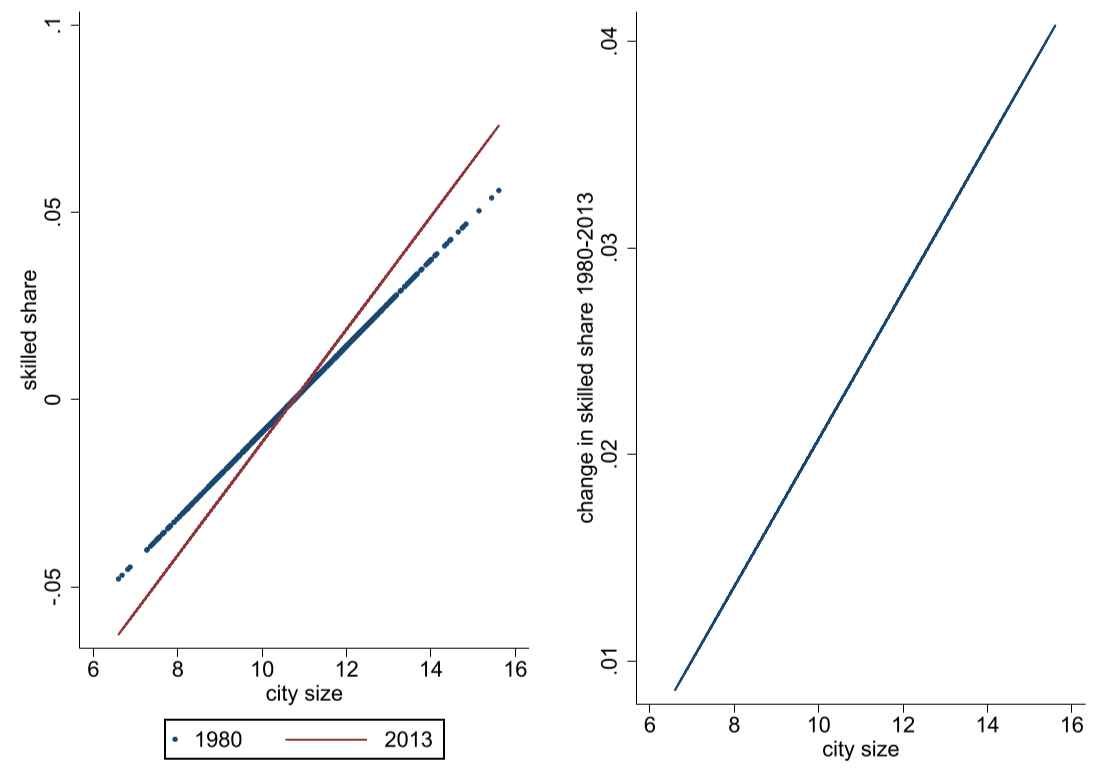
\includegraphics[scale=0.5]{domestic_fragmentation.png}
	\end{figure}
\end{frame}
%------------------------------------------------
\begin{frame}{Domestic fragmentation}{Jiao \& Tian 2021}
	\textbf{Settings}
	\begin{itemize}
		\item Two inputs: more skill-intensive knowledge inputs and relatively less skill-intensive standardized production;
		\item Worker heterogeneity: high-skill \& low-skill;
		\item Labor mobility;
		\item Fragmentation costs: the costs of communicating and coordinating due to the fragmentation.
	\end{itemize}
\end{frame}
%------------------------------------------------
\begin{frame}{Domestic fragmentation}{Jiao \& Tian 2021}
	\textbf{Manager’s optimization}
	\begin{itemize}
		\item First, choose where to live, which is also where she works or where the firm's headquarters are located;
		\item Second, choose the location of the production team;
		\item Finally, decide on the production scale (how many workers to hire).
	\end{itemize}
	$\Rightarrow$ Backward induction.
	\medskip

	\textbf{Worker's optimization}
	\begin{itemize}
		\item The same indirect utility across cities.
	\end{itemize}
\end{frame}
%------------------------------------------------
\subsection{Contractual Frictions and Multinational Firm Boundaries}
\begin{frame}[shrink]
	\transfade %fade in and fade out
	\tableofcontents[sectionstyle=show/shaded,subsectionstyle=show/shaded/hide]
	\addtocounter{framenumber}{-1}
\end{frame}
%------------------------------------------------
\begin{frame}{A temporary summary}
	\begin{block}{}
		Models above identify potential gains to fragment production across borders, or to use managerial know-how in a foreign country;
	\end{block}
	\begin{block}{}
		Not designed to explain
		\begin{itemize}
			\item Why these activities occur within firm's boundaries (i.e. foreign insourcing or FDI), rather than through arm's-length subcontracting, licensing, or outsourcing.
		\end{itemize}
	\end{block}
	\medskip
	$\Rightarrow$ They are \textcolor{red}{not theories of the MNE}, but \textcolor{red}{theories of the international production organization}.
\end{frame}
%------------------------------------------------
\begin{frame}{Internalization decision}
	\begin{block}{}
		Intel Corporation assembles most of its microchips in \textcolor{red}{wholly owned} subsidiaries in China, Costa Rica, Malaysia, and the Philippines.
	\end{block}
	\centering{
	v.s.
	}
	\begin{block}{}
		Nike subcontracts most of its manufacturing to \textcolor{red}{independent producers} in Thailand, Indonesia, Cambodia, and Vietnam.
	\end{block}
\end{frame}
%------------------------------------------------
\begin{frame}{Transaction cost theory}{Williamson 1975, 1985}
	\textbf{Settings}
	\begin{itemize}
		\item The investments are \textcolor{red}{relation-specific}. $\Rightarrow$ stickiness.
		\item At the renegotiation stage, parties cannot costlessly switch to alternative trading partners, partially locked into a bilateral relationship.
	\end{itemize}
	\medskip
	$\Rightarrow$ The combination of bilateral bargaining \& sunk costs may generate
	\begin{itemize}
		\item \textcolor{red}{ex-post inefficiencies} (e.g., inefficient termination or execution of the contract);
		\item \textcolor{red}{ex-ante or hold-up inefficiencies} (e.g., suboptimal provision of relationship-specific investments).
	\end{itemize}
\end{frame}
%------------------------------------------------
\begin{frame}{Transaction cost theory in international economics}
	\begin{block}{Ethier 1986}
		Vertical integration v.s. transaction at arm's length
	\begin{itemize}
		\item Transaction at arm's length cannot offer \textcolor{red}{quality-contingent} contracts to downstream producers or distributors.
		\item $\Rightarrow$ Headquarters cannot always devise a contract that ensures \textcolor{red}{ex-post} efficiency and extracts all surplus from contracting partners.
	\end{itemize}
	$\Rightarrow$ Integrating downstream producers may be better.
	\end{block}
	\begin{block}{McLaren 2000, Grossman \& Helpman 2002}
		Vertical integration v.s. outsourcing
	\begin{itemize}
		\item Suppliers undertake relationship-specific investments.
		\item In outsourcing, the final-good producer will hold up the supplier at the ex-post bargaining stage by offering him low payment.
	\end{itemize}
	$\Rightarrow$ The suppliers invest less \textcolor{red}{ex ante}, or pay cost to integrate.
	\end{block}
\end{frame}
%------------------------------------------------
\begin{frame}{Property rights theory}{Grossman \& Hart 1986}
	\begin{block}{}
		The transaction-cost approach is silent on the sources of vertical integration costs. \textcolor{red}{Or there is only one super-firm in the world\dots}
	\end{block}
	\begin{itemize}
		\item Ownership means the residual rights of control when contracts are incomplete.
		\item Vertical integration reduces the incentives of the integrated firm to make investments that are partially specific to the integrating firm,
		\item $\Rightarrow$ lowering the overall surplus of the relationship.
	\end{itemize}
\end{frame}
%------------------------------------------------
\begin{frame}{Property rights theory in international economics}{}
	\begin{block}{Antr\`as 2003}
		\begin{itemize}
			\item \textbf{Phenomenon:} Capital-intensive goods are transacted within firm boundaries, while labor-intensive goods are traded at arm's length.
			\item \textbf{Reason:}
			\begin{itemize}
				\item Noncontractible investments by headquarters are more capital-intensive.
				\item Those who invest more should have the residual rights of control to ensure incentives. (Grossman \& Hart 1986)
			\end{itemize}
			\item $\Rightarrow$ Integration beats outsourcing in headquarter intensive industries.
		\end{itemize}
	\end{block}
	\begin{block}{Antr\`as \& Helpman 2004}
		\begin{itemize}
			\item Allow for intra-industry heterogeneity;
			\item Only the most productive firms in an industry should be expected to vertically integrate their foreign suppliers.
		\end{itemize}
	\end{block}
\end{frame}
%------------------------------------------------
\section{Trading Firms and the Environment: An Application}
\begin{frame}[shrink]
	\transfade %fade in and fade out
	\tableofcontents[sectionstyle=show/shaded,subsectionstyle=show/shaded/hide]
	\addtocounter{framenumber}{-1}
\end{frame}
%------------------------------------------------
\begin{frame}{Trading firms and the environment}{Two tools}
	\textbf{Decomposition}
	\begin{itemize}
		\item Grossman \& Krueger (1993) and Copeland \& Taylor (1994) etc.
		\item Allow for both within-industry and within-firm changes in production.
	\end{itemize}
	\medskip
	\textbf{Partial equilibrium model}
	\begin{itemize}
		\item Firms choose the abatement level and decide whether to produce intermediate goods at home or outsource production abroad.
	\end{itemize}
\end{frame}
%------------------------------------------------
\begin{frame}{Trading firms and the environment}{New hypotheses from firm heterogeneity}
	\begin{itemize}
		\item The \textbf{\textcolor{red}{pollution reduction by rationalization hypothesis (PRR)}} links market share reallocations and selection effects in the Melitz (2003) model to changes in industry emissions.
		\medskip
		\item The \textbf{\textcolor{red}{distressed and dirty industry hypothesis (DDI)}} links changes in abatement and emission intensities to heightened foreign competition brought about by trade liberalization.
		\medskip
		\item The \textbf{\textcolor{red}{pollution offshoring hypothesis (POH)}} links firm-level decisions to offshore dirty intermediate inputs to trade liberalization with a partner that differs greatly in their pollution policy.
	\end{itemize}
\end{frame}
%-------------------------------------------------------------------------
%-------------------------------------------------------------------------
\subsection{The Mechanics of Pollution Emissions}
\begin{frame}[shrink]
	\transfade %fade in and fade out
	\tableofcontents[sectionstyle=show/shaded,subsectionstyle=show/shaded/hide]
	\addtocounter{framenumber}{-1}
\end{frame}
%------------------------------------------------
\begin{frame}{Industry-level decomposition}
	Consider an economy with aggregate pollution emissions $Z$ generated by $N$ industries. Each industry $i$ emits $Z_i$ units of pollution. $S_i$ denotes the scale of production in industry $i$.
	\begin{equation}
		Z=\sum_{i=1}^NS_iE_i,
	\end{equation}
	where $E_i=Z_i/S_i$ is the emission intensity of industry $i$.
	\begin{equation}
		\Rightarrow \hat{Z}=\hat{S}+\sum_{i=1}^N\Theta_i\hat{\Phi}_i+\sum_{i=1}^N\Theta_i\hat{E}_i,
	\end{equation}
	\begin{itemize}
		\item $S=\sum_{i=1}^NS_i$ is the economy-wide scale of output,
		\item $\Theta_i=Z_i/Z$ is the fraction of overall emissions $Z$ from industry $i$,
		\item $\Phi_i=S_i/S$ is industry $i$'s share of the economy's final output,
		\item $\hat{Z}=dZ/Z$, etc.
	\end{itemize}
\end{frame}
%------------------------------------------------
\begin{frame}{Industry-level decomposition}
	\begin{equation}\nonumber
		\hat{Z}=\hat{S}+\sum_{i=1}^N\Theta_i\hat{\Phi}_i+\sum_{i=1}^N\Theta_i\hat{E}_i
	\end{equation}
	\begin{itemize}
		\item $\hat{S}$: \textcolor{red}{scale effect}; changes in the overall level of economic activity.
		\item $\sum_{i=1}^N\Theta_i\hat{\Phi}_i$: \textcolor{red}{composition effect}; changes in the composition of economic activity across industries.
		\item $\sum_{i=1}^N\Theta_i\hat{E}_i$: \textcolor{red}{technique effect}; changes in the emission intensities of each industry.
	\end{itemize}
\end{frame}
%------------------------------------------------
\begin{frame}{Firm-level decomposition}
	Suppose each industry $i$ has a continuum of firms on the interval $[0,n_i]$. $z_i(n)$ denotes the emissions produced by firm $n$.
	\medskip

	Aggregate industry emissions are
	\begin{equation}
		Z_i=\int_0^{n_i}z_i(n)dn
	\end{equation}
	Denoting the value added produced by firm $i$ as $v_i(n)$, the scale of output in industry $i$ is
	\begin{equation}
		S_i=\int_0^{n_i}v_i(n)dn.
	\end{equation}
\end{frame}
%------------------------------------------------
\begin{frame}{Firm-level decomposition}
	The emission intensity of industry $i$ is
	\begin{equation}
		E_i=\frac{Z_i}{S_i}=\int_0^{n_i}e_i(n)\varphi_i(n)dn,
	\end{equation}
	where
	\begin{itemize}
		\item $e_i(n)=\frac{z_i(n)}{v_i(n)}$ is the emission intensity of firm $n$,
		\item $\varphi_i(n)=\frac{v_i(n)}{S_i}$ is the value-added share of firm $n$ in industry $i$.
	\end{itemize}
	\medskip
	\begin{equation}
		\Rightarrow \hat{E}_i=\int_0^{n_i}\hat{e}_i(n)\theta_i(n)dn + \int_0^{n_i}\hat{\varphi}_i(n)\theta_i(n)dn + n_i[\theta_i(n_i)-\varphi_i(n_i)]\hat{n}_i,
	\end{equation}
	where $\theta_i(n)=z_i(n)/Z_i$ is firm $n$'s share of emissions in industry $i$.
	\medskip
	\begin{itemize}
		\item $\int_0^{n_i}\hat{e}_i(n)\theta_i(n)dn$: changes in firm-level emission intensities;
		\item $\int_0^{n_i}\hat{\varphi}_i(n)\theta_i(n)dn$: industry composition effect;
		\item $n_i[\theta_i(n_i)-\varphi_i(n_i)]\hat{n}_i$: the impact of entry and exit.
	\end{itemize}
\end{frame}
%------------------------------------------------
\begin{frame}{Within-firm adjustment}
	Suppose firm $n$ produces output $y_i(n)$ by completing a set of $M_i(n)$ tasks. Let $T_i$ be the scale of task $i$. Assume the firm's output to be
	\begin{equation}
		y_i(n)=f_{i,n}(T_1,T_2,...,T_{M_i}).
	\end{equation}
	Let
	\begin{itemize}
		\item $\lambda_{ij}^I(n)$ be the fraction of task $j$ performed in-house by firm $n$,
		\item $\lambda_{ij}^d(n)$ be the fraction of task $j$ outsourced domestically,
		\item $\lambda_{ij}^*(n)$ be the fraction of task $j$ completed offshore.
	\end{itemize}
	\medskip
	We require
	\begin{equation}
		\lambda_{ij}^I(n) + \lambda_{ij}^d(n) + \lambda_{ij}^*(n) = 1.
	\end{equation}
\end{frame}
%------------------------------------------------
\begin{frame}{Within-firm adjustment}
	\begin{equation}
		p_i(n)y_i(n)=[1+\mu_i(n)]\sum_{j=1}^{M_i} w_{ij}(n)T_{ij}(n),
	\end{equation}
	where
	\begin{itemize}
		\item $p_i(n)$ is the price used to value output,
		\item $w_{ij}$ is the price used to value a unit of task $j$,
		\item $\mu_i(n)$ is the rate at which firm $n$ marks up the unit cost of tasks.
	\end{itemize}
	\medskip
	The value added produced by firm $n$ is
	\begin{equation}
		\begin{aligned}
			v_i(n)&=p_i(n)y_i(n)-\sum_{j=1}^{M_i}[1-\lambda_{ij}^I(n)]w_{ij}(n)T_{ij}(n) \\
			&=\sum_{j=1}^{M_i}\lambda_{ij}^I(n)w_{ij}(n)T_{ij}(n) + \mu_i(n)\sum_{j=1}^{M_i}w_{ij}(n)T_{ij}(n).
		\end{aligned}
	\end{equation}
\end{frame}
%------------------------------------------------
\begin{frame}{Within-firm adjustment}
	Denote the firm's domestic emission intensity of task $j$ (per unit value) as $e_{ij}(n)$. The firm's domestic emissions level from task $j$ is then
	\begin{equation}
		z_{ij}(n) = e_{ij}(n)\lambda_{ij}^I(n)w_{ij}(n)T_{ij}(n).
	\end{equation}
	The total level of pollution emitted domestically by firm $n$ in industry $i$ is
	\begin{equation}
		z_i(n)=\sum_{j=1}^{M_i}z_{ij}(n)=\sum_{j=1}^{M_i}\lambda_{ij}^I(n)e_{ij}(n)w_{ij}(n)T_{ij}(n),
	\end{equation}
	so the overall emission intensity of firm $n$ (per dollar of value added) is
	\begin{equation}
		e_i(n)=\frac{z_i(n)}{v_i(n)}=\frac{\sum_{j=1}^{M_i}\lambda_{ij}^I(n)e_{ij}(n)\sigma_{ij}(n)}{\sum_{j=1}^{M_i}\lambda_{ij}^I(n)\sigma_{ij}(n)+\mu_i(n)},
	\end{equation}
	where
	\begin{equation}
		\sigma_{ij}(n) = \frac{w_{ij}(n)T_{ij}(n)}{\sum_{j=1}^{M_i}w_{ij}(n)T_{ij}(n)}
	\end{equation}
	is the share of task $j$ in the total cost of all tasks.
\end{frame}
%------------------------------------------------
\begin{frame}{Within-firm adjustment}
	Decompose the emission intensity of firm $n$ in industry $i$:
	\begin{small}
		\begin{equation}
			\begin{aligned}
				\hat{e}_i(n)&=\underbrace{ \sum_{j=1}^{M_i}\theta_{ij}(n)\hat{e}_{ij}(n)}_{\text{technique effect}} + \underbrace{\sum_{j=1}^{M_i}[\theta_{ij}(n)-\varphi_{ij}(n)]\hat{\sigma}_{ij}(n)}_{\text{composition / reorganization effect}} \\
				&\underbrace{-\sum_{j=1}^{M_i}\frac{\lambda_{ij}^d(n)}{\lambda_{ij}^I(n)}[\theta_{ij}(n)-\varphi_{ij}(n)]\hat{\lambda}_{ij}^d(n)}_{\text{domestic outsourcing effect}} \\
				&\underbrace{-\sum_{j=1}^{M_i}\frac{\lambda_{ij}^*(n)}{\lambda_{ij}^I(n)}[\theta_{ij}(n)-\varphi_{ij}(n)]\hat{\lambda}_{ij}^*(n)}_{\text{offshoring effect}} \underbrace{-\varphi_{i\mu}(n)\hat{\mu}_i(n)}_{\text{markup effect (-)}},
			\end{aligned}
		\end{equation}
	\end{small}
	\begin{itemize}
		\item $\theta_{ij}=z_{ij}(n)/z_i(n)$ is task $j$ 's in-house emissions share in firm $n$,
		\item $\varphi_{ij}(n)$ is the firm's in-house production share of task $j$ in value added,
		\item $\varphi_{i\mu}(n)$ is the share of revenue from markups in value added.
	\end{itemize}
\end{frame}
%------------------------------------------------
\begin{frame}{Within-firm adjustment}
	\begin{small}
	\begin{equation}
		\begin{aligned}
			\hat{Z} &= {\textcolor{brown}{\hat{S}}} + {\textcolor{blue}{\sum_{i=1}^N\Theta_i\hat{\Phi}_i}} + {\textcolor{red}{\sum_{i=1}^N\Theta_i\int_0^{n_i}\hat{\varphi}_i(n)\theta_i(n)dn + \sum_{i=1}^N\Theta_in_i[\theta_i(n)-\varphi_i(n_i)]\hat{n}_i}} \\
			&+ {\textcolor{red}{\sum_{i=1}^N\Theta_i\int_0^{n_i}\left[\sum_{j=1}^{M_i}[\theta_{ij}(n)-\varphi(n)]\hat{\sigma}_{ij}(n)\right]\theta_i(n)dn}} \\
			&- {\textcolor{red}{\sum_{i=1}^N\Theta_i\int_0^{n_i}\left[\sum_{j=1}^{M_i}\frac{\lambda_{ij}^d(n)}{\lambda_{ij}^I(n)}[\theta_{ij}(n)-\varphi_{ij}(n)]\hat{\lambda}_{ij}^d(n)\right]\theta_i(n)dn}} \\
			&- {\textcolor{red}{\sum_{i=1}^N\Theta_i\int_0^{n_i}\left[\sum_{j=1}^{M_i}\frac{\lambda_{ij}^*(n)}{\lambda_{ij}^I(n)}[\theta_{ij}(n)-\varphi_{ij}(n)]\hat{\lambda}_{ij}^*(n)\right]\theta_i(n)dn}} \\
			&+ {\textcolor{red}{\sum_{i=1}^N\Theta_i\int_0^{n_i}\left[\sum_{j=1}^{M_i}\theta_{ij}(n)\hat{e}_{ij}(n)\right]\theta_i(n)dn - \sum_{i=1}^N\Theta_i\int_0^{n_i}[\varphi_i(n)\hat{\mu}_i(n)]\theta_i(n)dn}}
		\end{aligned}
	\end{equation}
	\end{small}
\end{frame}
%-------------------------------------------------------------------------
%-------------------------------------------------------------------------
\subsection{Trade, Firm Heterogeneity and the Environment}
\begin{frame}[shrink]
	\transfade %fade in and fade out
	\tableofcontents[sectionstyle=show/shaded,subsectionstyle=show/shaded/hide]
	\addtocounter{framenumber}{-1}
\end{frame}
%------------------------------------------------
\begin{frame}{Technology and costs}
	\textbf{Settings: (Melitz 2003)}
	\begin{itemize}
		\item Produce differentiated goods; monopolistic competition
		\item CES preference
		\item Firms must pay a fixed entry cost to obtain a productivity draw and a fixed cost to engage in any production.
		\item Firms have to pay an additional fixed cost $F_e$ (in terms of labor) to export and incur variable shipping costs.
	\end{itemize}
\end{frame}
%------------------------------------------------
\begin{frame}{Technology and costs}
	The firm produces final goods by using a Leontief technology to assemble a continuum of intermediates $x(j),j\in[0,1]$.
	\medskip

	Each intermediate good $j$ is produced with a CES production technology using clean and dirty inputs:
	\begin{equation}
		x(L,D;j)=\gamma[a_j^{1-\delta}L^\delta+b_j^{1-\delta}D^\delta]^{1/\delta},
	\end{equation}
	where $\delta<1$, $a_j>0$, and $b_j>0$.
	\begin{itemize}
		\item $L$ is a clean input (such as labor) with factor price $w$
		\item $D$ is a dirty input available at price $r$
		\item $\gamma>0$ is a productivity parameter
		\item $j$ increases in the dirty input intensity of intermediates $b_j/a_j$.
	\end{itemize}
\end{frame}
%------------------------------------------------
\begin{frame}{Technology and costs}
	Firms can pay a fixed cost $A$ to invest in abatement technology. So the pollution emissions are
	\begin{equation}
		z=g(A)D,
	\end{equation}
	where $g(A)$ is decreasing in $A$ and $0\leq g(A)\leq 1$.
	\medskip

	The government regulates pollution with an emission tax $\tau$, so the full price $\tau_D$ for the dirty input is
	\begin{equation}
		\tau_D=r+\tau g(A).
	\end{equation}
\end{frame}
%------------------------------------------------
\begin{frame}{Technology and costs}
	Firms decide to produce intermediates in-house or offshore abroad by comparing relative costs. Assume that the pollution charges at home are relatively high, \footnote{$*$ denotes foreign variables.}
	\begin{equation}
		\frac{\tau_D}{w}>\frac{\tau_D^*}{w^*}.
	\end{equation}
	\medskip
	The domestic firm offshores intermediates for which
	\begin{equation}
			[1+\kappa]c^*(w^*,\tau_D^*;j)<c(w,\tau_D;j),
	\end{equation}
	where
	\begin{equation}
		c(w,\tau_D;j) = \frac{1}{\gamma}\left[a_jw^{1-\sigma}+b_j\tau_D^{1-\sigma}\right]^{\frac{1}{1-\sigma}}.
	\end{equation}
	\begin{itemize}
		\item $\kappa>0$ shows the variable costs of outsourcing; $\sigma=1/[1-\delta]$.
	\end{itemize}
\end{frame}
%------------------------------------------------
\begin{frame}{Technology and costs}
	\begin{equation}
		[1+\kappa]c^*(w^*,\tau_D^*;j)<c(w,\tau_D;j),\quad \Leftrightarrow\quad\frac{w}{w^*}>\left[1+\kappa\right]T_j
	\end{equation}
	where
	\begin{equation}
		T_j\equiv \frac{\gamma}{\gamma^*}\left[\frac{1+\frac{b_j}{a_j}[\tau^*_D/w^*]^{1-\sigma}}{1+\frac{b_j}{a_j}[\tau_D/w]^{1-\sigma}}\right]^{1/[1-\sigma]}
	\end{equation}
	measures the role of environmental policy and emission intensities in determining the cost of foreign production relative to home production.
	\medskip
	\begin{itemize}
		\item Intermediates on the interval $(j_0,1]$ are offshored because of the relatively stringent environmental policy at home.
	\end{itemize}	
\end{frame}
%------------------------------------------------
\begin{frame}[label=figure1]{Technology and costs}
	\begin{figure}[h]
		\centering
		The Decision to Offshore

		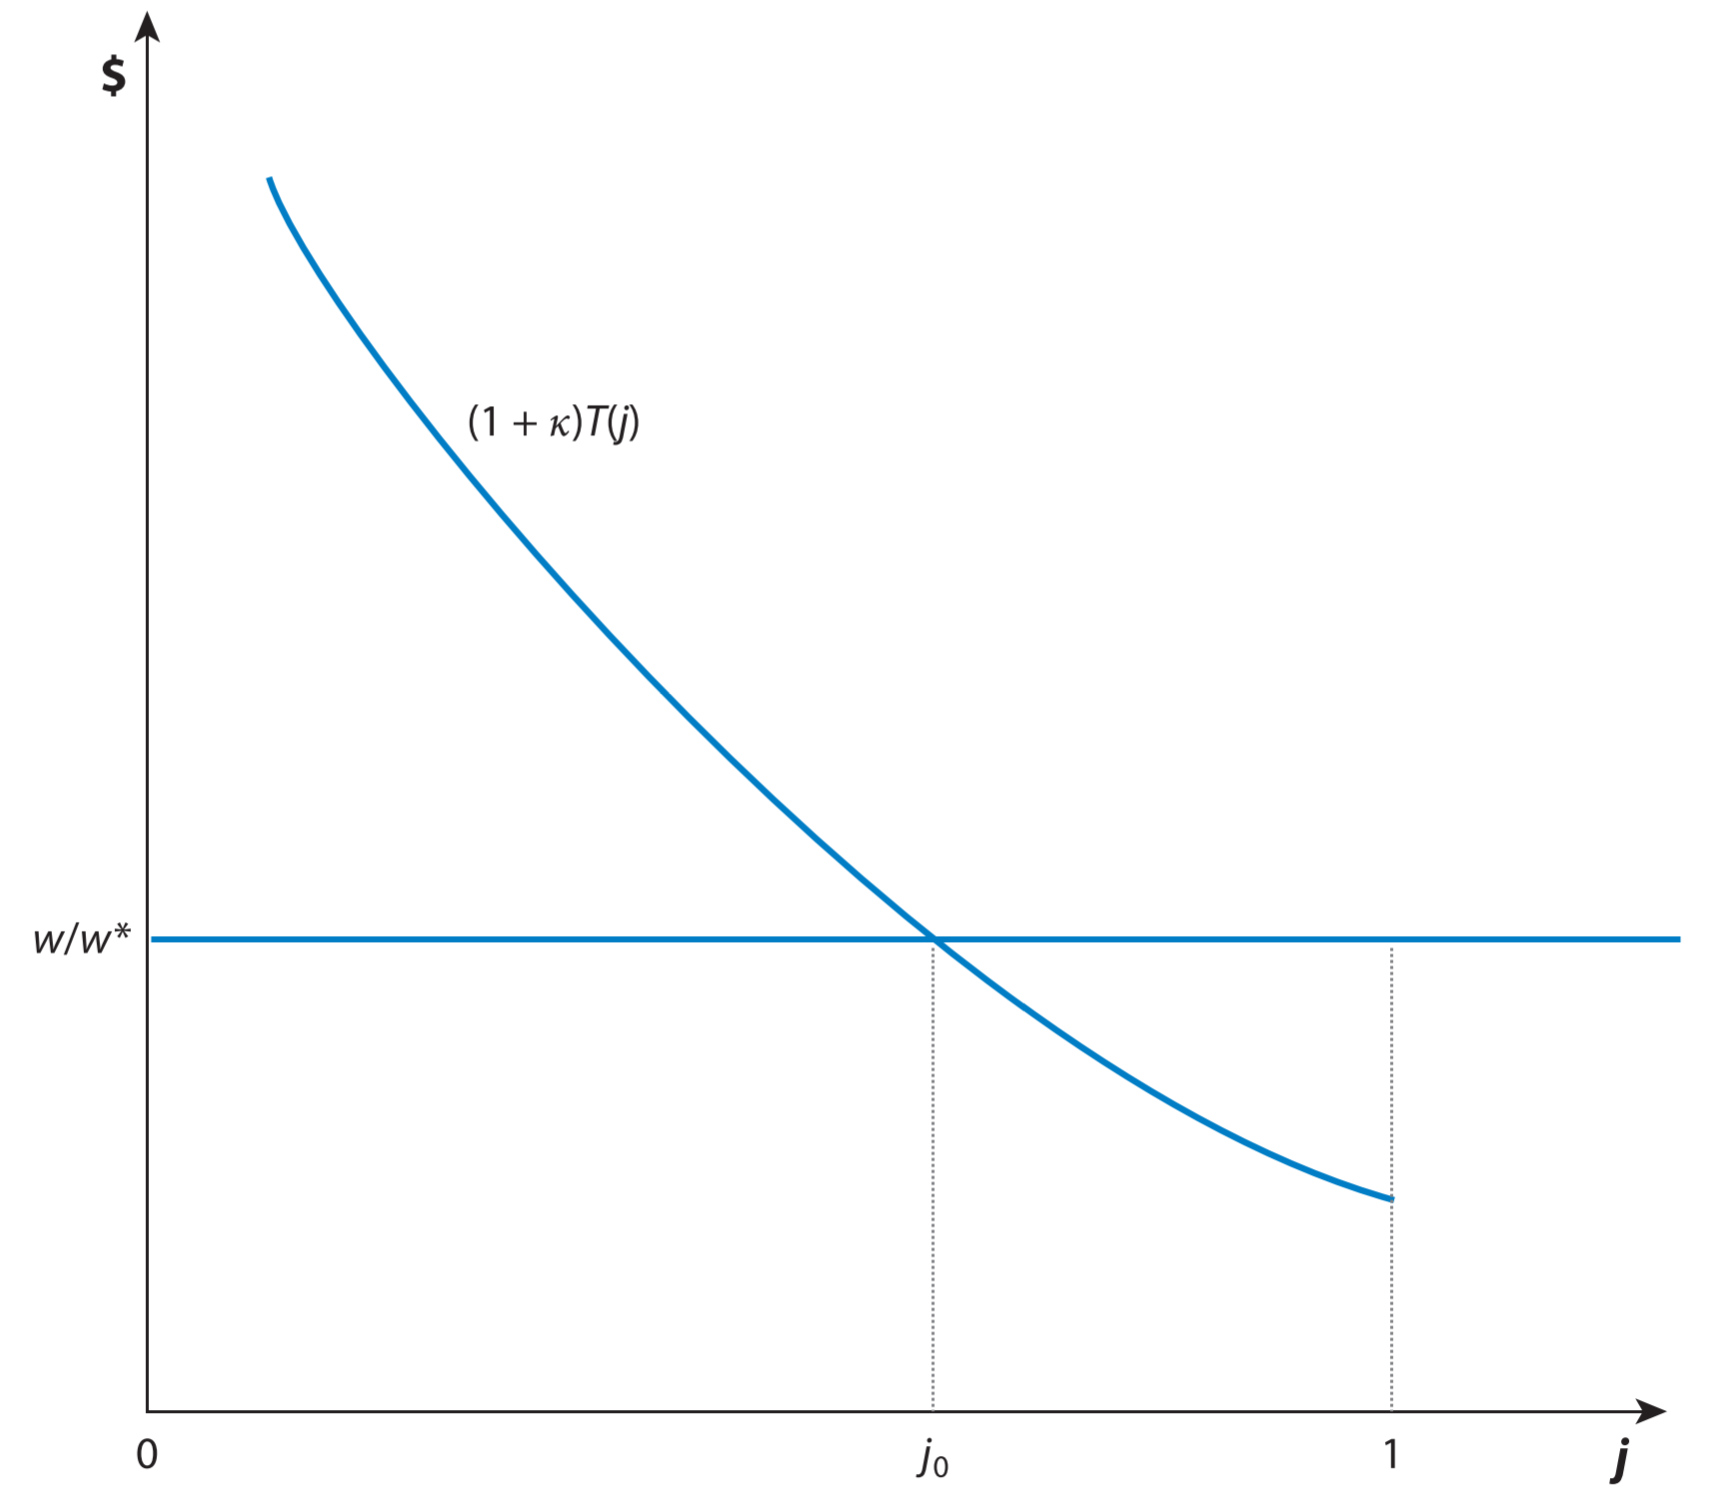
\includegraphics[scale=0.23]{figure1.png}
	\end{figure}
	Source: Cherniwchan et al 2017.
	\hfill\hyperlink{wfa}{\beamergotobutton{With-firm Adjustment}}
	\hfill\hyperlink{poh}{\beamergotobutton{POH}}
\end{frame}
%------------------------------------------------
\begin{frame}{Technology and costs}
	Finally, the firm minimizes costs by choosing abatement:
	\begin{equation}
		C(A) = \int^{j_0}_0 c(w,\tau_D(A);j)dj + \int_{j_0}^1 c^*(w^*,\tau_D^*;j)dj.
	\end{equation}
	\begin{equation}
		\Rightarrow \quad \tilde{C}(A)=\min_A \{yC(A)+A\}.
	\end{equation}
	\begin{itemize}
		\item Higher emission charges increase the incentive to abate, as do higher output levels.
		\item For given output levels, more productive firms abate less.
	\end{itemize}
	\medskip
	$\Rightarrow$ If a firm's output were to increase more than in proportion to an increase in productivity, then abatement would rise.
\end{frame}
%------------------------------------------------
\begin{frame}{The effects of trade liberalization}{Across-firm adjustments}
	To focus on adjustments across firms, assume that
	\begin{itemize}
		\item firm-level emission intensities are constant (abatement is fixed, no outsourcing, and the price of dirty inputs is fixed)
		\item only one industry.
	\end{itemize}
\end{frame}
%------------------------------------------------
\begin{frame}{The effects of trade liberalization}{Across-firm adjustments}
	\begin{figure}[h]
		\centering
		The Decision to Export and the Effects of Trade Liberalization

		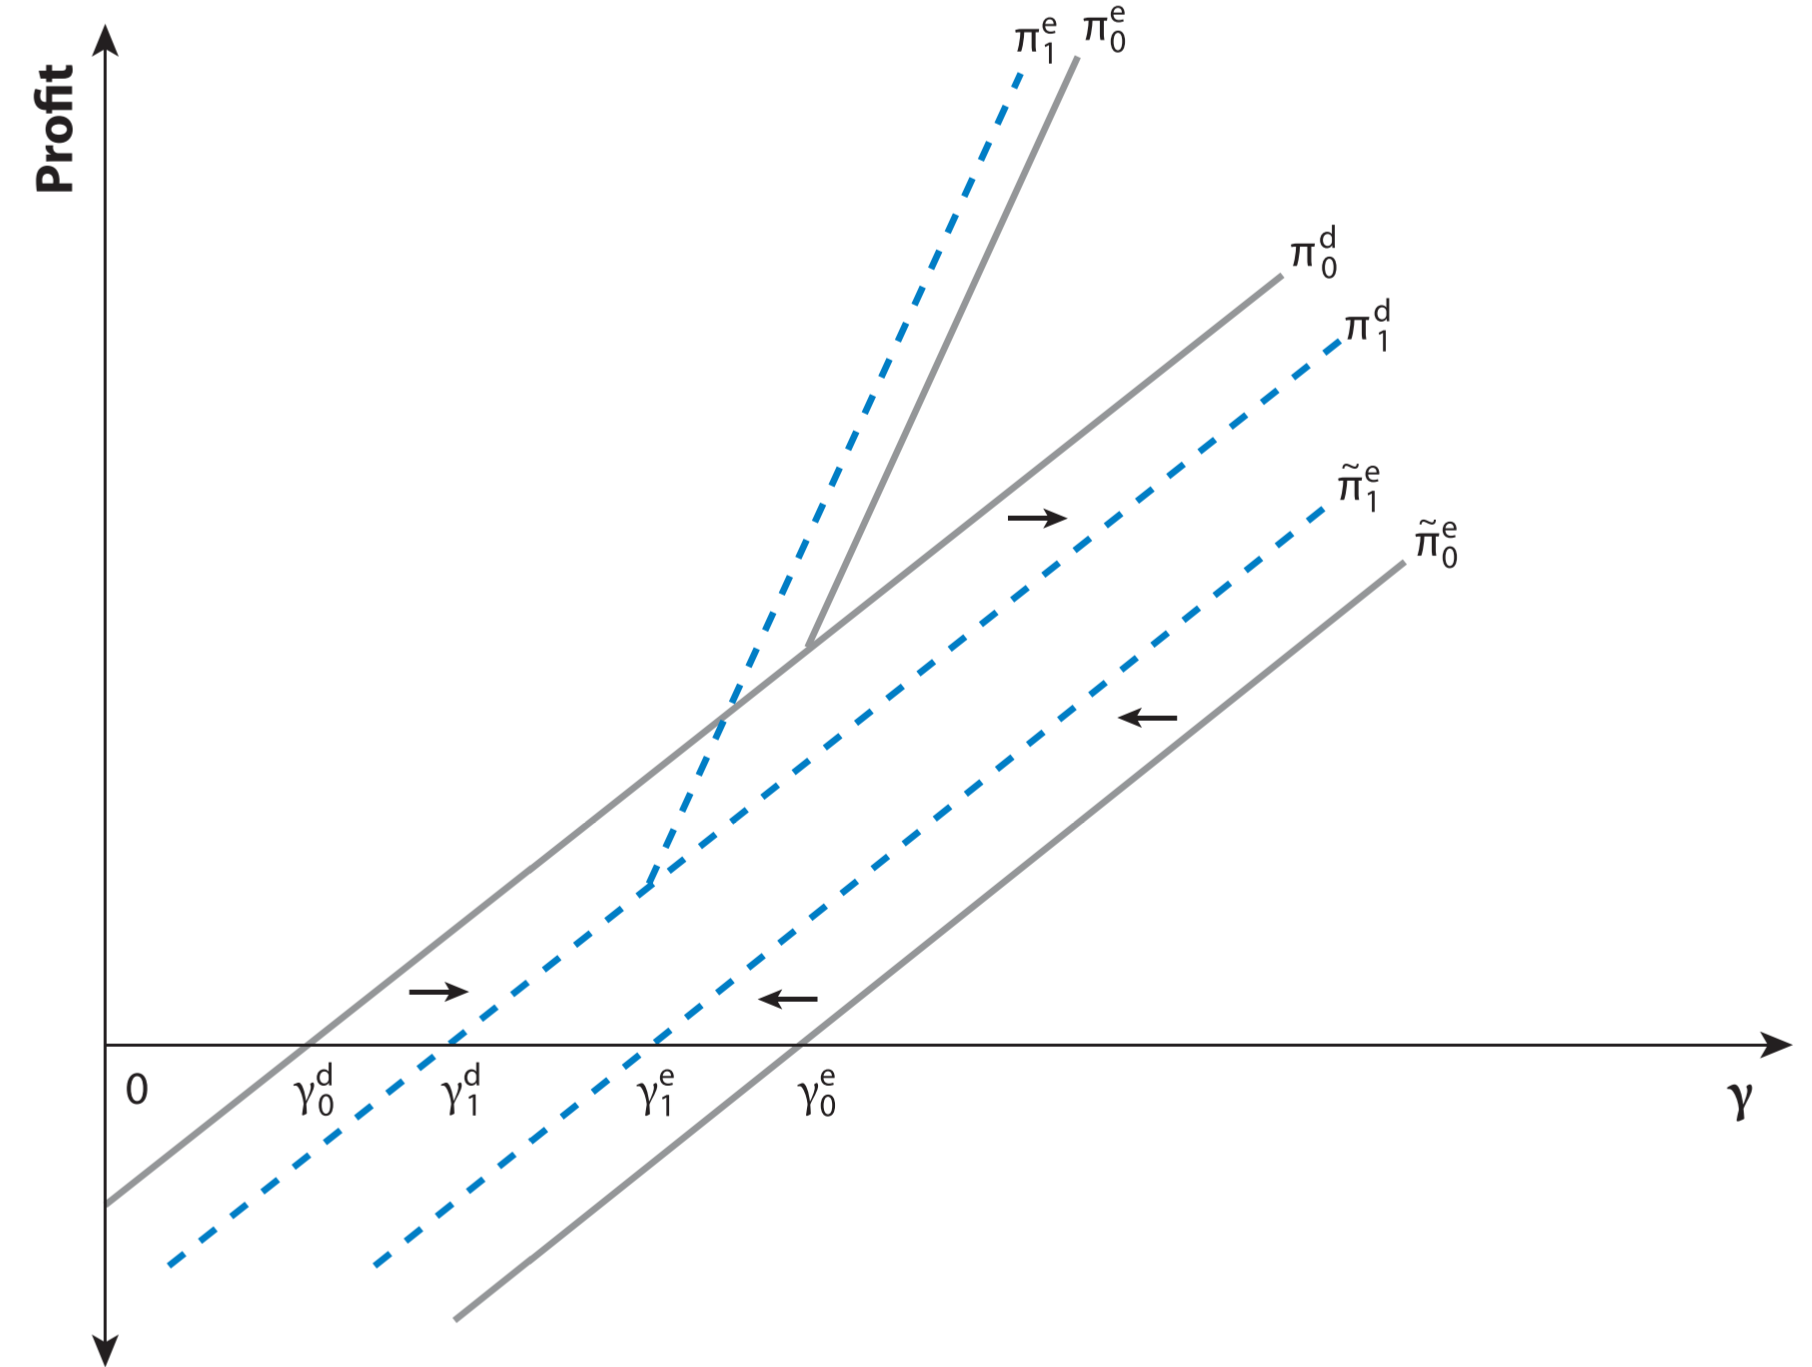
\includegraphics[scale=0.25]{figure2.png}
	\end{figure}
	Source: Cherniwchan et al. 2017.
\end{frame}
%------------------------------------------------
\begin{frame}{The effects of trade liberalization}{Across-firm adjustments}
	Because emission intensities are constant, the effect of trade liberalization on emissions is
	\begin{equation}
		dZ=\underbrace{dS}_{\text{scale effect (+)}} + \underbrace{\int_0^{n_0}e(n)d\varphi(n)dn}_{\text{market share
		reallocation (-)}} + \underbrace{\varphi(n)[e(n)-E]dn_0}_{\text{selection effects (-)}},
	\end{equation}
	where $n_0$ is the marginal firm.
	\medskip

	$\Rightarrow$ \textbf{Pollution Reduction by Rationalization (PRR) hypothesis:} trade liberalization lowers industry emissions because a mix of exit, entry, and market share reallocations overwhelms the positive scale effects
	created by new export opportunities.
\end{frame}
%------------------------------------------------
\begin{frame}[label=wfa]{The effects of trade liberalization}{Within-firm adjustments}
	For a single firm, $z=ve$. Hence,
	\begin{equation}
		\hat{z} = \hat{v} + \hat{e},
	\end{equation}
	where
	\begin{equation}
		\hat{e}=\underbrace{\int_0^{j_0}\theta_j\hat{e}_jdj}_{\text{emission intensity change}} + \underbrace{[\theta_{j_0}-\varphi_{j_0}]d_{j_0}}_{\text{offshoring}}.
	\end{equation}
	\hfill\hyperlink{figure1}{\beamergotobutton{Figure}}
\end{frame}
%------------------------------------------------
\begin{frame}{The effects of trade liberalization}{Emission intensities and abatement}
	\textbf{Key question:} whether firms' endogenous abatement choices reinforce the rationalization and selection effects that operate at the industry level.

	\medskip
	\textbf{Three complications}
	\begin{enumerate}
		\item Sensitive to the demand structure:
		\begin{itemize}
			\item Cao et al. (2016) use a preference structure by Melitz \& Ottaviano (2008) and show that more productive firms may abate less.
		\end{itemize}
		\item Investment in abatement need not lower emission intensities.
		\begin{itemize}
			\item Direct effect: emissions per unit of the dirty input fall.
			\item Classic rebound effect: abatement encourages substitution towards dirty inputs.
		\end{itemize}
		\item Winners v.s. losers: exporters expand output and become cleaner, while surviving domestic firms reduce output and thus abatement.
	\end{enumerate}
\end{frame}
%------------------------------------------------
\begin{frame}{The effects of trade liberalization}{Emission intensities and abatement}
	Endogenous abatement complicates the set of adjustments and may introduce a negative but novel potential outcome from trade liberalization.

	\medskip
	\begin{itemize}
		\item \textbf{Distressed and Dirty Industry (DDI) hypothesis:} trade liberalization increases industry emissions because of reductions in pollution control or abatement that downsize as a result of trade.
	\end{itemize}
\end{frame}
%------------------------------------------------
\begin{frame}[label=poh]{The effects of trade liberalization}{Offshoring dirty inputs}
	\textbf{Pollution Offshoring Hypothesis (POH):} domestic firms become cleaner not because they have reduced the emission intensity, but because they have shifted the dirtiest parts of production abroad.\footnote{Unlike PHH, POH is more subtle as it concerns the fragmentation of production — only the dirtiest parts of the production process are shifted abroad.}\hfill\hyperlink{figure1}{\beamergotobutton{Figure}}
	\medskip

	\textbf{Two implications}
	\begin{itemize}
		\item Abatement investments and offshoring dirty intermediates are substitutes for firms to react to more stringent environmental policy.
		\item If the POH holds, trade liberalization may reduce the incentives for pollution abatement investments.
	\end{itemize}
\end{frame}
%-------------------------------------------------------------------------
%-------------------------------------------------------------------------
\section{Conclusion}
\begin{frame}[shrink]
	\transfade %fade in and fade out
	\tableofcontents[sectionstyle=show/shaded,subsectionstyle=show/shaded/hide]
	\addtocounter{framenumber}{-1}
\end{frame}
%------------------------------------------------
\begin{frame}{Conclusion}
	\begin{itemize}
		\item The development of trade theory is, to a large extent, the process of increasingly deepening specialization, from industry-level to firm-level and then to production-stage-level.
		\medskip
		\item Corresponding to this development, heterogeneity at different levels takes place. New sources of gains from trade and the possibility of distortions emerge.
	\end{itemize}
\end{frame}
%------------------------------------------------
%------------------------------------------------
\begin{frame}
	\addtocounter{framenumber}{-1}
	\Huge{\centerline{\textit{The End}}}
\end{frame}
%-------------------------------------------------------------------------
\begin{frame}{Reference}
	\addtocounter{framenumber}{-1}
	\footnotesize
	Antr\`as, P. (2003). Firms, contracts, and trade structure. \textit{The Quarterly Journal of Economics}, 118(4), 1375-1418.

	Antr\`as, P., \& Helpman, E. (2004). Global sourcing. \textit{Journal of Political Economy}, 112(3), 552-580.

	Antr\`as, P., Garicano, L., \& Rossi-Hansberg, E. (2006). Offshoring in a knowledge economy. \textit{The Quarterly Journal of Economics}, 121(1), 31-77.

	Baldwin, R. E., \& Robert-Nicoud, F. (2008). Trade and growth with heterogeneous firms. \textit{Journal of International Economics}, 74(1), 21-34.

	Cherniwchan, J., Copeland, B. R., \& Taylor, M. S. (2017). Trade and the environment: New methods, measurements, and results. \textit{Annual Review of Economics}, 9, 59-85.

	Copeland, B. R., \& Taylor, M. S. (1994). North-South trade and the environment. \textit{The Quarterly Journal of Economics}, 109(3), 755-787.

	Ethier, W. J. (1986). The multinational firm. \textit{The Quarterly Journal of Economics}, 101(4), 805-833.

	Grossman, S. J., \& Hart, O. D. (1986). The costs and benefits of ownership: A theory of vertical and lateral integration. \textit{Journal of Political Economy}, 94(4), 691-719.
\end{frame}
\begin{frame}{Reference}
	\addtocounter{framenumber}{-1}
	\footnotesize
	Grossman, G. M., \& Helpman, E. (2002). Integration versus outsourcing in industry equilibrium. \textit{The Quarterly Journal of Economics}, 117(1), 85-120.

	Grossman, G. M., \& Krueger, A. B. (1995). Economic growth and the environment. \textit{The Quarterly Journal of Economics}, 110(2), 353-377.

	Grossman, G. M., \& Rossi-Hansberg, E. (2008). Trading tasks: A simple theory of offshoring. \textit{American Economic Review}, 98(5), 1978-97.

	Grossman, G. M., \& Rossi-Hansberg, E. (2012). Task trade between similar countries. \textit{Econometrica}, 80(2), 593-629.

	Jiao, Y., \& Tian, L. (2021). Geographic fragmentation in a knowledge economy. Working Paper.

	Jones, R. W., \& Kierzkowski, H. (1991). \textit{The role of services in production and international trade} (No. ARTICLE).

	Jones, R. W., \& Kierzkowski, H. (2001). \textit{Globalization and the consequences of international fragmentation} (No. ARTICLE).

	Kremer, M., \& Maskin, E. (1996). \textit{Wage Inequality and Segregation by Skill} (No. 5718). National Bureau of Economic Research, Inc.
\end{frame}
\begin{frame}{Reference}
	\addtocounter{framenumber}{-1}
	\footnotesize
	Kremer, M., \& Maskin, E. (2006). Globalization and inequality.

	Lucas Jr, R. E. (1978). On the size distribution of business firms. \textit{The Bell Journal of Economics}, 508-523.

	McLaren, J. (2000). " Globalization" and vertical structure. \textit{American Economic Review}, 90(5), 1239-1254.
	
	Melitz, M. J. (2003). The impact of trade on intra-industry reallocations and aggregate industry productivity. \textit{Econometrica}, 71(6), 1695-1725.
	
	Rodr\'iguez-Clare, A. (2010). Offshoring in a ricardian world. \textit{American Economic Journal: Macroeconomics}, 2(2), 227-58.

	Williamson, O. E. (1975). \textit{Markets, Hierarchies: Analysis, Antitrust Implications}. New York: Free Press.

	Williamson, O. E. (1985). \textit{The Economic Institutions of Capitalism}. New York: Free Press.

	Yi, K. M. (2003). Can vertical specialization explain the growth of world trade?. \textit{Journal of Political Economy}, 111(1), 52-102.
\end{frame}


\end{document} 